\subsection{Data Partitioning and Organization}
%kNN join is one type of spatial joins. It is a computation-intensive operation, because we should compute the pairwise 
%distance for every elements in R 
%and in S. So parallel processing is a good way for this operation especially when the size and dimension of data are big. 
%\TODO{we start directly with mapreduce, why not with centralized approaches? -- Discussion Needed --}
First attempts to compute kNN efficiently in shared-memory focused on particular data organizations, such that the neighbor set can be pruned and neighbor sorting is 
performed faster. 
%\TODO{check}. 
In the most popular methods, data are 
usually indexed using a tree structure like $B^+$-Tree \cite{DBLP:journals/tods/JagadishOTYZ05} or R-Tree \cite{MuX}. But as we 
target big data, shared-memory centric solutions cannot be easily applied to a shared-nothing platform as MapReduce. 
Instead, the dataset need to be separated into several sets, called partitions, such that, ideally, each partition is 
independent from others. It is nonetheless possible to use efficient data structures to improve local searching in a partition. 

As in any MapReduce computation, the data partition 
strategy will strongly impact CPU, network communication and disk usage, which in turn will impact the overall processing 
time\cite{DBLP:conf/hpcc/SongMHMYL13}
. 
The key to improve the performance is to preserve spatial locality of objects when decomposing data for tasks 
\cite{Zhou:1998:DPP:594718.594759}. This 
means making a coarse clustering in order to produce a reduced set of neighbors that are candidates for the final result. Intuitively,
the goal is to have a partitioning of data such as an element in a partition of $R$ will have its nearest neighbors 
in only one partition of $S$. More precisely, what we want is:

For every partition $R_i$ ($\cup_{i}R_i=R$), find a corresponding partition $S_j$ ($\cup_{j}S_j=S$), where
\begin{center}
$kNN(R_i \ltimes S) = kNN(R_i \ltimes S_j)$, and, 
$kNN(R \ltimes S) = \bigcup kNN(R_i \ltimes S_j)$
\end{center}
which means that, not only it is possible to compute kNN for each element of $R_i$ in a single $S_j$, but also the concatenation of the results for all $R_i$ is equal to the global kNN join.

%This is why we need a data partition strategy before processing the real kNN job. 
%Data partitioning is thus a key challenge for 
%parallel spatial join 
%processing. It is not only studied in kNN problem processing on top of MapReduce, but also studied by other parallel spatial 
%join processing such as in
%\cite{Zhou:1998:DPP:594718.594759}. However, depending on the kind of the problem and on the processing platform, the partitioning
%method varies.  
%So the methods which can partition data into shared-nothing subset such as some k-means methods or projection based methods are usually used for data organization in MapReduce. 
In this section, we present two partition methods that enable to separate the 
dataset into shared-nothing subsets while preserving locality information.
 
%In this section, we will first analyze the load balance problem for partitioning, then we will introduce several partitioning methods mainly classified into two categories. 

%As we described above, for the kNN join for two datasets R and S, the ideal situation is to firstly find out the partition for R, then generate the corresponding partition of S.
%Here we only list 2 types of the partition methods based on this guiding ideology have been used in running kNN join on MapReduce.

\subsubsection{Distance Based Partitioning}
The first partitioning method is based on Voronoi diagram, a method to divide the space into disjoint cells. The main property of this method 
is that every point in a cell is
closer to the pivot of this cell than to any other pivot. Because this method relies on the distance metric, it is naturally used to solve neighborhood problems. More formally, the 
definition of a Voronoi cell is as follow:
\begin{myDef}
Given a set of disjoint pivots: P = $\left\{ p_1, p_2, ..., p_i, ..., p_n \right\}$, the Voronoi Cell of $p_i$ $\left(0 < 
i \leq n \right)$ is: $
\forall$ i $\neq$ j, $VC\left(p_i\right) = \left\{p \| d\left(p, p_i\right) \leq d\left(p, p_j\right) \right\}$. 
\end{myDef}

\begin{figure}[t]
\centering
\scalebox{0.20}{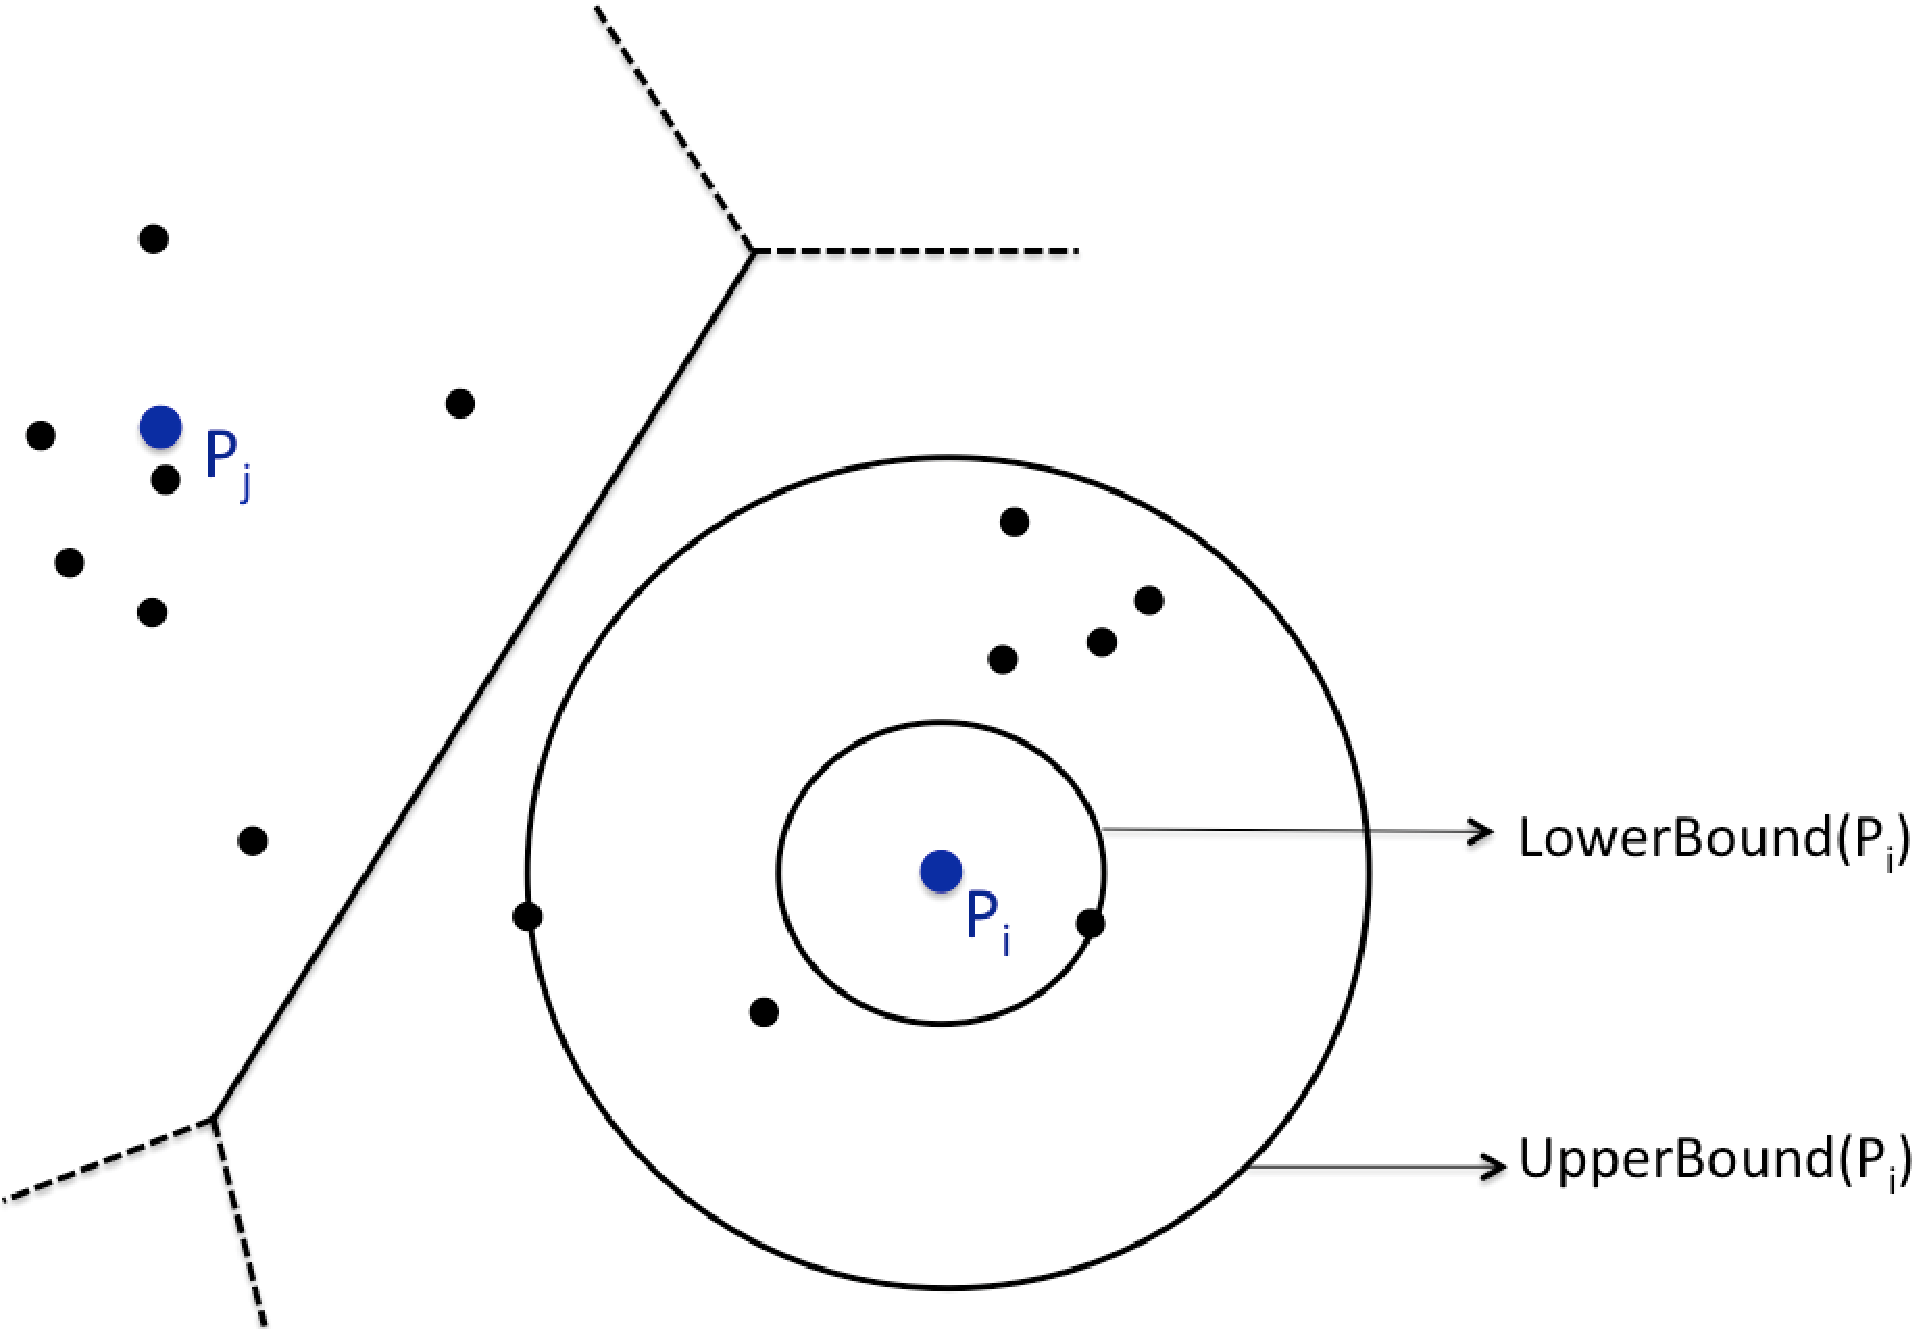
\includegraphics{res/voronoi-partition.pdf}}
\caption{Voronoi based partitioning for pivots $P_i$ and $P_j$ \label{voronoi_partition_figure}}
\end{figure}

Paper \cite{Lu:2012:EPK:2336664.2336674} gives a method to partition the dataset $R$ and $S$ using Voronoi diagram. 
After having identified the pivots in $R$ (as seen in the preprocessing section - \ref{data_preprocessing}), they compute the distance between every point and 
the pivots, and put the considered point into the cell of the closest pivot. This will  naturally give a partitioning of data. Afterwards, they also 
calculate, for each cell of $R$,
the upper (resp. lower) bound of the partition which corresponds to the sphere determined by the furthest (resp. closest) point (in $S$) from the pivot in 
the cell of $R$. Such bounds enable to quickly find the correct partition $S_j$ for a given partition $R_i$.
This data partitioning principle is shown in Figure~\ref{voronoi_partition_figure} where two pivots $P_i$ and $P_j$ have been chosen from the dataset.
%of the nearest neighbors in $S$ for each partition of $R$ to find out the corresponding partition of $S$ \TODO{rewrite}.

The main problem of this method is that it requires computing the distance of all elements to the pivots. Also, the distribution of the input data might 
not be known in advance. Hence, the pivots will have to be recomputed if the data changes, which limits dynamicity. Also, there is no 
guarantee that all cells will have an equal number of elements because of potential data skew. This can have a negative impact on the overall performance
because of load balancing issues.  

\subsubsection{Size Based Partitioning} 

Another type of partitioning method aims at dividing the data into some equal size partitions while preserving their locality 
information. \cite{Zhang:2012:EPK:2247596.2247602} proposes a partitioning strategy based on $z$-value described in the 
previous section. 
%They first compute the $z$-value of every points in $R$. 
In 
order to make every partition of $R$ have a similar number of objects, a sampling is first performed. They claim that the $n$ quantiles 
($n$ is equal to the number of partitions) of the sampling data is an unbiased estimation of the boundary point of each partition, with a
standard deviation $\leq$ $\epsilon\left|R\right|$ $\left( \epsilon > 0\right)$.
After having partitioned $R$ this way, the same sampling strategy is applied to $S$. For each of the boundary points 
of all $R_i$, the corresponding $k^{th}$ nearest neighbor is identified in $S$. These points are then used as boundary points of the corresponding $S_i$.
As a consequence, the partitions of $S$ are overlapping such that for any given point in $R$, all the $k$ nearest neighbors can always be found in a 
single partition of $S$. An example of $z$-value based partition is  given in Figure~\ref{projection_partition_figure}.
\begin{figure}[t]
\centering
\scalebox{0.20}{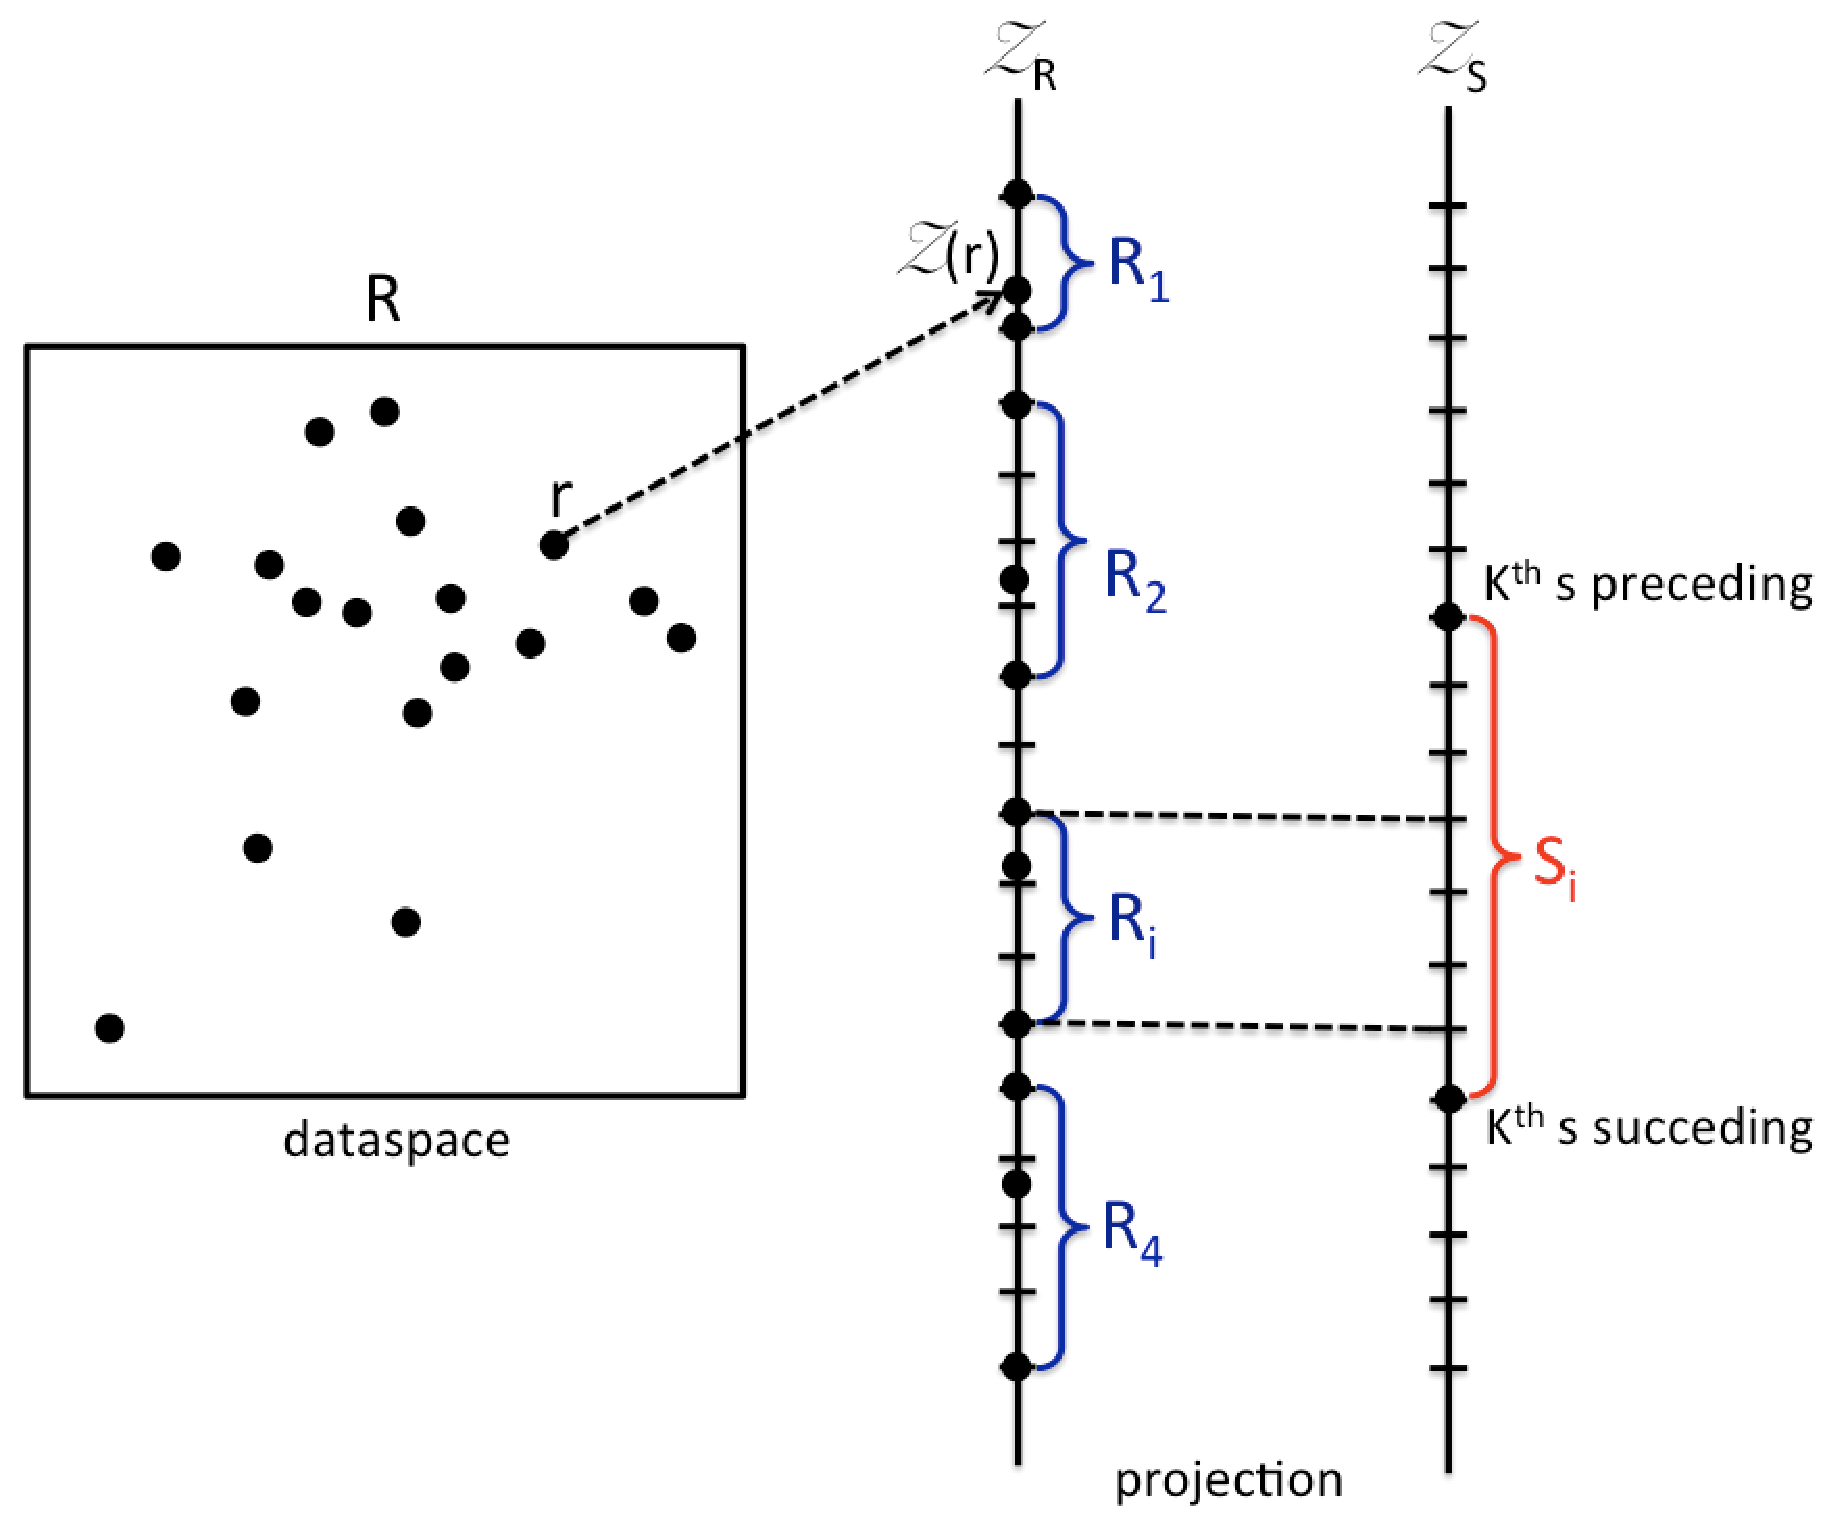
\includegraphics{res/projection-partition.pdf}}
\caption{$z$-value based partitioning \label{projection_partition_figure}}
\end{figure}
This method is likely to produce a substantially equivalent number of objects in each partition. 

Another similar size based partitioning method can be applied for datasets that are preprocessed with \emph{Locality Sensitive Hashing}, as illustrated in 
Figure~\ref{lsh_partition_figure}. With this method, the elements of $R$ that are projected to $LSH(R)$, are divided into 
quasi-equal size partitions using a sampling technique. The same technique can be applied to $S$ and $LSH(S)$. 



%To conclude this section, two kinds of partitioning method can be applied. The first kind, that we have called distance based partitioning, enables a 
%straight-forward partitioning of the raw data around pivots. However, this methods does not guarantee that all the $k$ nearest neighbors 
%will be found in a single partition. The number of partitions of $S$ needed to satisfy query points in a given partition of $R$ is dependent on the number 
%of partitions and the number of elements in each of them \TODO{check}. On the other hand, the second kind of partitioning method, called size based 
%partitioning, ensures to find all the $k$ 
%nearest neighbors in a constant number of partitions, for example, three partitions at maximum in \cite{Zhang:2012:EPK:2247596.2247602} (the one 
%considered and the ones directly to the left and to the right \TODO{not clear, the text above claim they need a single partition}). 
%To conclude this section, two kinds of partitioning methods can be applied for separating data while preserving their locality relationship. 
The strategy of partitioning will impact directly the number of tasks and the amount of computation. Distance based methods aim at dividing the close objects together by pre-selecting some pivots. Size based methods want to separate objects into equal size zones in which the points are ordered.
Regarding the implementation, \cite{Lu:2012:EPK:2336664.2336674} uses a MapReduce job to 
perform the partitioning. In \cite{Zhang:2012:EPK:
2247596.2247602}, both data preprocessing and data partitioning are completed in one MapReduce job.

\begin{figure}[t]
\centering
\scalebox{0.25}{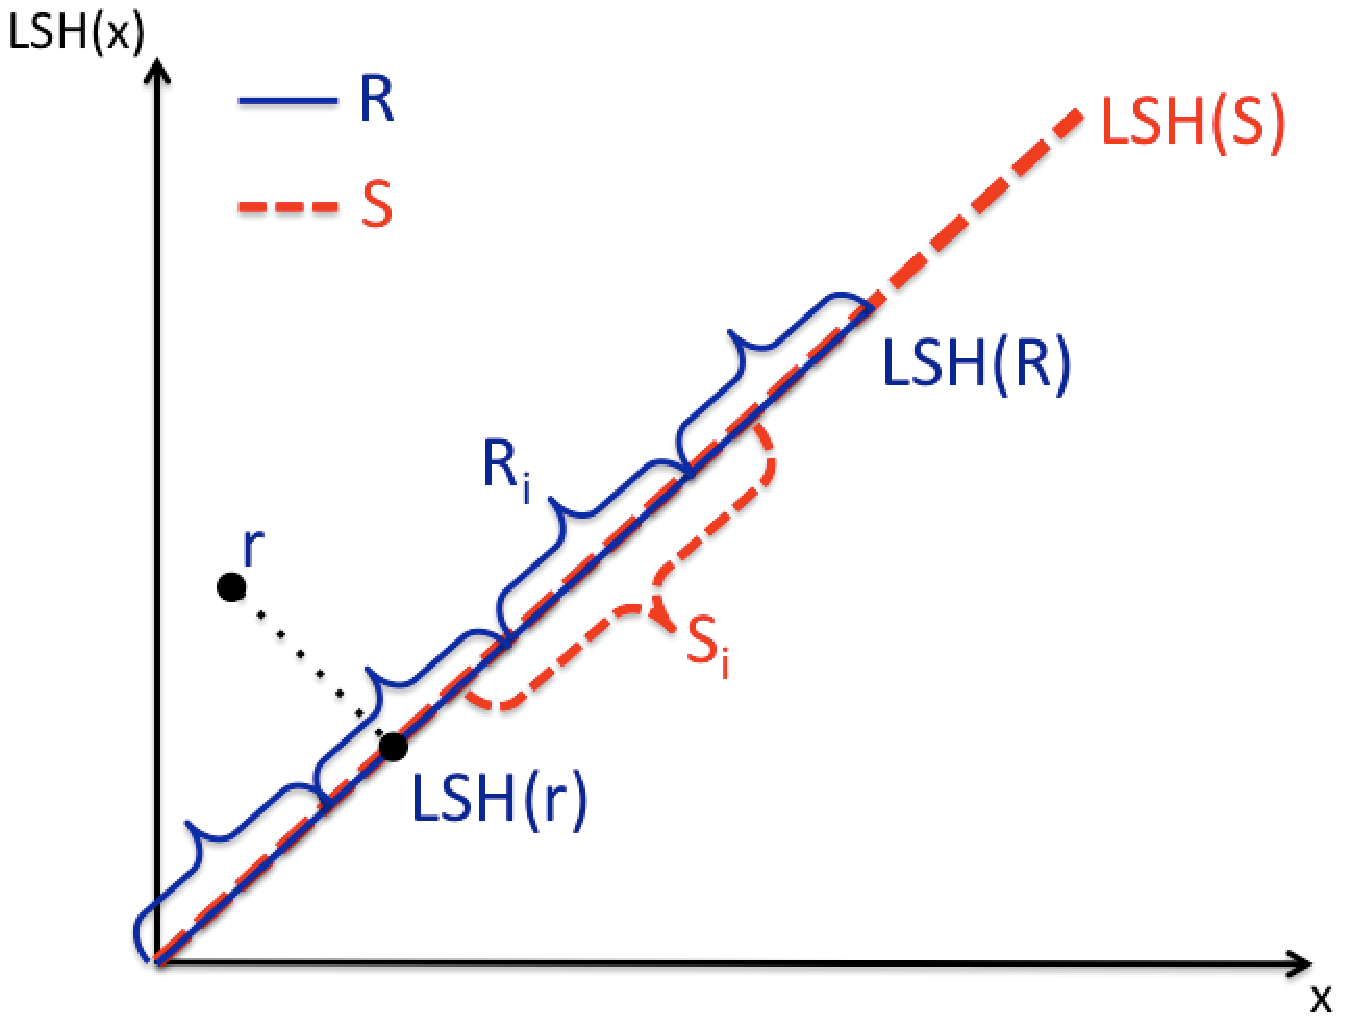
\includegraphics{res/lsh-partition.pdf}}
\caption{LSH based partitioning \label{lsh_partition_figure}}
\end{figure}
%LSH is an approximate approach and }. 
%Although it's more probable for the related objects to have the same hash value than the distance ones, normally one hash function can not guarantee
%the accuracy. We often need a group of hash functions to generate multiple hash tables to avoid the conflict probability of close objects.  
